
\documentclass[tikz,convert={convertexe={magick.exe}}]{standalone}
\usetikzlibrary{shapes.misc}

\begin{document}
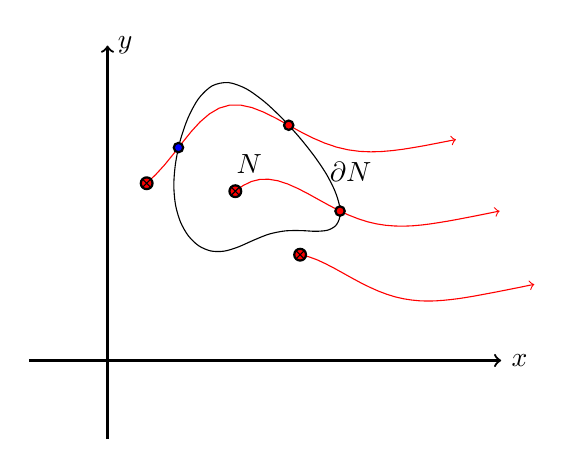
\begin{tikzpicture}


\tikzstyle atom=[circle, draw, inner sep=1.2pt, fill=red, thick]

\draw[thick, ->] (-1,0) -- (5,0) node[right] {$x$};
\draw[thick, ->] (0,-1) -- (0,4) node[right] {$y$};


\draw[] plot[smooth cycle] coordinates{(2.887,2.155) (2.782,2.363) (2.633,2.586) (2.448,2.821) (2.235,3.058) (2.002,3.279) (1.763,3.450) (1.534,3.530) (1.329,3.488) (1.157,3.327) (1.022,3.080) (0.923,2.792) (0.863,2.499) (0.842,2.223) (0.864,1.974) (0.927,1.758) (1.027,1.583) (1.158,1.457) (1.313,1.391) (1.482,1.389) (1.663,1.443) (1.853,1.527) (2.051,1.605) (2.256,1.646) (2.459,1.650) (2.643,1.641) (2.794,1.655) (2.898,1.713) (2.949,1.820) (2.945,1.971)};
\draw[red,->] (1.623,2.150)--(1.722,2.222)--(1.826,2.273)--(1.935,2.300)--(2.048,2.302)--(2.166,2.282)--(2.288,2.242)--(2.414,2.186)--(2.541,2.121)--(2.669,2.050)--(2.798,1.979)--(2.925,1.912)--(3.051,1.852)--(3.175,1.803)--(3.297,1.763)--(3.417,1.735)--(3.535,1.717)--(3.651,1.708)--(3.765,1.706)--(3.878,1.711)--(3.990,1.721)--(4.101,1.735)--(4.212,1.752)--(4.322,1.770)--(4.432,1.790)--(4.542,1.811)--(4.651,1.832)--(4.761,1.854)--(4.870,1.876)--(4.980,1.898);
\node[atom,fill=red] at (2.953,1.898) {};
\node[atom, inner sep=1.5pt] at (1.623,2.150) {};
\node[cross out, draw, inner sep=1.5pt] at (1.623,2.150) {};
\draw[red,->] (2.446,1.344)--(2.551,1.319)--(2.659,1.280)--(2.769,1.229)--(2.881,1.171)--(2.993,1.109)--(3.106,1.046)--(3.218,0.986)--(3.329,0.931)--(3.439,0.882)--(3.547,0.841)--(3.654,0.808)--(3.759,0.784)--(3.862,0.768)--(3.964,0.758)--(4.064,0.755)--(4.164,0.757)--(4.262,0.764)--(4.360,0.774)--(4.458,0.786)--(4.555,0.801)--(4.651,0.817)--(4.748,0.835)--(4.844,0.853)--(4.940,0.871)--(5.036,0.890)--(5.132,0.909)--(5.228,0.928)--(5.324,0.948)--(5.420,0.967);
\node[atom, inner sep=1.5pt] at (2.446,1.344) {};
\node[cross out, draw, inner sep=1.5pt] at (2.446,1.344) {};
\draw[red,->] (0.497,2.251)--(0.614,2.363)--(0.728,2.488)--(0.839,2.625)--(0.950,2.767)--(1.061,2.905)--(1.175,3.030)--(1.294,3.132)--(1.418,3.205)--(1.550,3.243)--(1.689,3.244)--(1.835,3.212)--(1.986,3.153)--(2.141,3.076)--(2.298,2.989)--(2.455,2.903)--(2.610,2.825)--(2.763,2.759)--(2.912,2.709)--(3.059,2.675)--(3.202,2.656)--(3.342,2.650)--(3.481,2.654)--(3.618,2.666)--(3.753,2.683)--(3.889,2.705)--(4.023,2.728)--(4.157,2.754)--(4.291,2.780)--(4.425,2.806);
\node[atom,fill=blue] at (0.901,2.704) {};
\node[atom,fill=red] at (2.301,2.988) {};
\node[atom, inner sep=1.5pt] at (0.497,2.251) {};
\node[cross out, draw, inner sep=1.5pt] at (0.497,2.251) {};


\node[right] at (2.7,2.4) {$\partial N$};

\node[] at (1.8,2.5) {$N$};



\end{tikzpicture}
\end{document}